\documentclass[a4paper,english,12pt]{article}
\usepackage{%
	amsfonts,%
	amsmath,%	
	amssymb,%
	amsthm,%
	algorithm,%
	babel,%
	bbm,%
	etex,%
	%biblatex,%
	caption,%
	centernot,%
	color,%
	dsfont,%
	enumerate,%
	epsfig,%
	epstopdf,%
	geometry,%
	graphicx,%
	hyperref,%
	latexsym,%
	mathtools,%
	multicol,%
	pgf,%
	pgfplots,%
	pgfplotstable,%
	pgfpages,%
	proof,%
	psfrag,%
	subfigure,%	
	tikz,%
	ulem,%
	url%
}	
\usepackage[noend]{algpseudocode}
\usepackage[mathscr]{eucal}
\usepgflibrary{shapes}
\usetikzlibrary{%
  	arrows,%
	backgrounds,%
	chains,%
	decorations.pathmorphing,% /pgf/decoration/random steps | erste Graphik
	decorations.text,%
	matrix,%
  	positioning,% wg. " of "
  	fit,%
	patterns,%
  	petri,%
	plotmarks,%
  	scopes,%
	shadows,%
  	shapes.misc,% wg. rounded rectangle
  	shapes.arrows,%
	shapes.callouts,%
  	shapes%
}

\theoremstyle{plain}
\newtheorem{thm}{Theorem}[section]
\newtheorem{lem}[thm]{Lemma}
\newtheorem{prop}[thm]{Proposition}
\newtheorem{cor}[thm]{Corollary}

\theoremstyle{definition}
\newtheorem{defn}[thm]{Definition}
\newtheorem{conj}[thm]{Conjecture}
\newtheorem{exmp}[thm]{Example}
\newtheorem{assum}[thm]{Assumptions}
\newtheorem{axiom}[thm]{Axiom}

\theoremstyle{remark}
\newtheorem{rem}{Remark}
\newtheorem{note}{Note}
\newtheorem{fact}{Fact}

\newcommand{\norm}[1]{\left\lVert#1\right\rVert}
\newcommand{\indep}{\!\perp\!\!\!\perp}
\DeclarePairedDelimiter\abs{\lvert}{\rvert}%
\newcommand\numberthis{\addtocounter{equation}{1}\tag{\theequation}}
\newcommand{\tr}{\operatorname{tr}}
\newcommand{\R}{\mathbb{R}}
\newcommand{\N}{\mathbb{N}}
\newcommand{\E}{\mathbb{E}}
\newcommand{\Z}{\mathbb{Z}}
\newcommand{\B}{\mathscr{B}}
\newcommand{\C}{\mathcal{C}}
\newcommand{\T}{\mathscr{T}}
\newcommand{\F}{\mathcal{F}}
\newcommand{\G}{\mathcal{G}}
%\newcommand{\ba}{\begin{align*}}
%\newcommand{\ea}{\end{align*}}
\DeclareMathOperator*{\argmax}{arg\,max}
\renewcommand{\qedsymbol}{$\blacksquare$}
\makeatletter
\def\BState{\State\hskip-\ALG@thistlm}
\makeatother

\makeatletter
\def\th@plain{%
  \thm@notefont{}% same as heading font
  \itshape % body font
}
\def\th@definition{%
  \thm@notefont{}% same as heading font
  \normalfont % body font
}
\makeatother
\date{}
\title{Lecture 26: Expectation Maximization(EM algorithm)}
\date{April 12, 2016}
\author{}
\begin{document}
\maketitle
\textbf{AIM}: Suppose we get only partial observations/samples from a parameterized population, then how can we perform efficient maximum likelihood parameter estimation?\\
\textbf{Applications:}
\begin{enumerate}
\item Machine Learning
\item Clustering (Unsupervised learning)
\item Bio-informatics, Genomics, Speech processing (Baum-Welch algorithm)
\end{enumerate}
\section{Estimating Mixtures of Gaussians (MoG)}
The MoG model is a joint distribution on $(\boldsymbol{x},z)$ with $\boldsymbol{x} \in \R^{d}, z\in [k] $ and $z$ has multinomial distribution,  $$z\sim \text{Multinomial Distribution}(\pmb{\phi})$$ 
i.e., Multinomial$\left[[\phi_1, \phi_2, ... \phi_k]^T\right]$ with $\phi_i\geq0 ~; ~\sum_{j=1}^{k}\phi_j=1.$
Given $z=j$, the random vector $\boldsymbol{x}$ is Gaussian distributed $\boldsymbol{x}|(z=j) \sim \mathcal{N}(\boldsymbol{\mu}_j, \Sigma_j)$. Here, $\pmb{\phi}$ is the mixture distribution, $ \{\boldsymbol{\mu}_j\}$ is the cluster center and $ \{ \Sigma_j\}$ is the cluster size.
\begin{exmp}\label{exmp:1}
For $d=k=2$, let 
\begin{equation*}
\boldsymbol{\mu}_1=\begin{bmatrix}
1\\
1
\end{bmatrix}
~;~ \boldsymbol{\mu}_2=\begin{bmatrix}
-1\\
-1
\end{bmatrix},
\end{equation*}
\begin{equation*}
\Sigma_1=\Sigma_2=I_2,~\mbox{and}~\pmb{\phi}=
\begin{bmatrix}
    0.5   &0.5
    \end{bmatrix}.
\end{equation*}
Here, cluster concentration is uniform as seen in Fig. \ref{fig:Example 1}, and roughly centers of clusters are $\boldsymbol{\mu}_1$ and $\boldsymbol{\mu}_2$.
\begin{figure}[h]
\centering
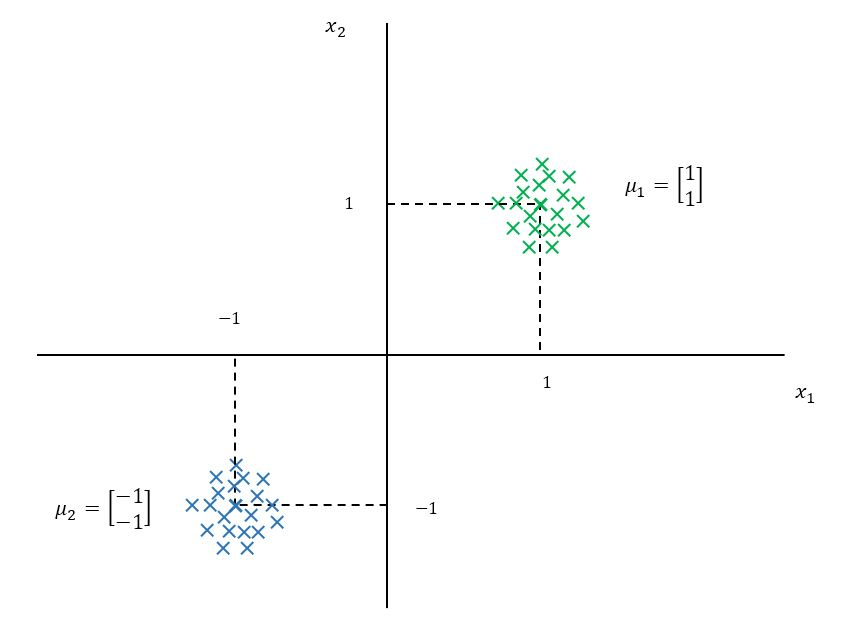
\includegraphics[width=0.9\linewidth]{Figures/Lect26fig1.jpg}
\caption[rdr]{Example 1}
\label{fig:Example 1}
\end{figure}
\end{exmp}
\begin{exmp}\label{exmp:2}
For $d=k=2$, let \begin{equation*}
\boldsymbol{\mu}_1=\begin{bmatrix}
1\\
1
\end{bmatrix}
~;~ \boldsymbol{\mu}_2=\begin{bmatrix}
-1\\
-1
\end{bmatrix},
\end{equation*}
\begin{equation*}
\Sigma_1=\Sigma_2=I_2,~\mbox{and}~\pmb{\phi}=
\begin{bmatrix}
    0.25   &0.75
    \end{bmatrix}.
\end{equation*}
Since the distribution is non-uniform, cluster density is also different (see Fig. \ref{fig:Example 2}).
\begin{figure}[h]
\centering
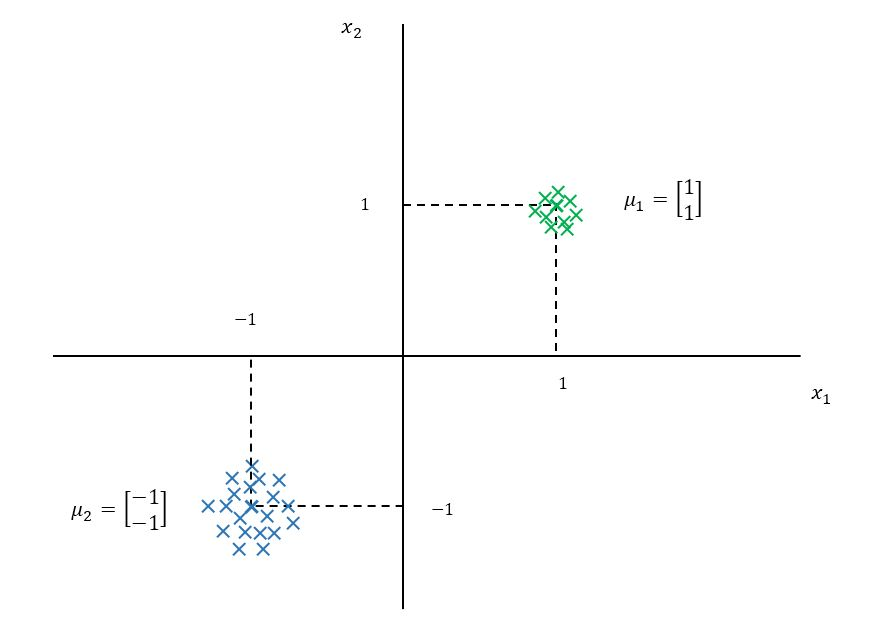
\includegraphics[width=0.9\linewidth]{Figures/Lect26fig2.jpg}
\caption[rdr]{Example 2}
\label{fig:Example 2}
\end{figure}
\end{exmp}
Let us define parameter 
\begin{equation}
\theta\equiv(\pmb{\phi}, \underbrace{\boldsymbol{\mu}_1, \boldsymbol{\mu}_2, ...,\boldsymbol{\mu}_k}_{\boldsymbol{\mu}}, \underbrace{\Sigma_1, \Sigma_2, ...,\Sigma_k}_{\boldsymbol{\Sigma}}).
\end{equation}
Suppose we only observe $\boldsymbol{x_1},\boldsymbol{x_2},...,\boldsymbol{x_m}\in \R^d$ where $(\boldsymbol{x_i},z_i)\overset{iid}{\sim }$ mixture of Gaussians with parameter $\theta$ (here, $z_i$ is called ``latent variable"). The goal is to find a ``maximum likelihood" estimate of $\theta$.
\begin{align}
\theta_{\text{MLE}}&=\underset{\theta\equiv\{\pmb{\phi},\boldsymbol{\mu},\boldsymbol{\Sigma}\}}{\arg\max}\sum_{i=1}^{m}\log{p\left(\boldsymbol{x_i}|\pmb{\phi},\boldsymbol{\mu},\boldsymbol{\Sigma}\right)}\\
&=\underset{\{\pmb{\phi},\boldsymbol{\mu},\boldsymbol{\Sigma}\}}{\arg\max}\sum_{i=1}^{m}\log{\sum_{z_i\in[k]}p\left(\boldsymbol{x_i},z_i|\pmb{\phi},\boldsymbol{\mu},\Sigma\right)}\\
&=\underset{\{\pmb{\phi},\boldsymbol{\mu},\boldsymbol{\Sigma}\}}{\arg\max} \sum_{i=1}^{m}\log{\sum_{z_i=1}^{k}\phi(z_i)f(\boldsymbol{x_i}|(z=z_i))}
\end{align}
where $\boldsymbol{x_i}|(z=z_i)\sim\mathcal{N}\left(\boldsymbol{\mu}_{z_i},\Sigma_{z_i}\right)$. This optimization is impossible to solve in closed form over $\{\pmb{\phi},\boldsymbol{\mu},\boldsymbol{\Sigma}\}$. However, MLE solution is easy if $\{ z_i \}_{i=1}^{m}$ were observed. 
\subsubsection*{Case: $\{ z_i \}_{i=1}^{m}$ are observed}
In this case,
\begin{align}
\tilde{\theta}_{\text{MLE}}&=\underset{\{\pmb{\phi},\boldsymbol{\mu},\boldsymbol{\Sigma}\}}{\arg\max}\sum_{i=1}^{m}\log{p\left(\boldsymbol{x_i},z_i|\pmb{\phi},\boldsymbol{\mu},\Sigma\right)}\\
&=\underset{\{\pmb{\phi},\boldsymbol{\mu},\boldsymbol{\Sigma}\}}{\arg\max} \sum_{i=1}^{m}\left[\log{\phi(z_i)}+\underset{\sim\mathcal{N}\left(\boldsymbol{\mu}_{z_i},\Sigma_{z_i}\right)}{\log{f(\boldsymbol{x_i}|z_i)}}\right]\\
&=\underset{\{\pmb{\phi},\boldsymbol{\mu},\boldsymbol{\Sigma}\}}{\arg\max} \sum_{i=1}^{m}\sum_{j=1}^{k}\mathds{1}_{\{z_i=j\}}\left[\log{\phi(j)}+\underset{\sim\mathcal{N}\left(\boldsymbol{\mu}_{j},\Sigma_{j}\right)}{\log{f(\boldsymbol{x_i}|z_i=j)}}\right]\\
&=\underset{\{\pmb{\phi},\boldsymbol{\mu},\boldsymbol{\Sigma}\}}{\arg\max} \left[\sum_{j=1}^{k}\log{\phi(j)}\sum_{i=1}^{m}\mathds{1}_{\{z_i=j\}}+\sum_{j=1}^{k}\sum_{i=1}^{m}\mathds{1}_{\{z_i=j\}}\underset{\sim\mathcal{N}\left(\boldsymbol{\mu}_{j},\Sigma_{j}\right)}{\log{f(\boldsymbol{x_i}|z_i=j)}}\right]\\
&=\{\tilde{\pmb{\phi}},\tilde{\boldsymbol{\mu}},\tilde{\Sigma }\}
\end{align}
where,
\begin{align}
\tilde{\mu}_j&=\frac{\sum_{i=1}^{m}\mathds{1}_{\{z_i=j\}}x_i}{\sum_{i=1}^{m}\mathds{1}_{\{z_i=j\}}}\\
\tilde{\Sigma}_j&=\frac{1}{\sum_{i=1}^{m}\mathds{1}_{\{z_i=j\}}}\sum_{i=1}^{m}\mathds{1}_{\{z_i=j\}}\left(x_i-\overset{\sim}{\mu}_j\right)\left(x_i-\overset{\sim}{\mu}_j\right)^T\\
\tilde{\phi}_j&=\frac{1}{m}\sum_{i=1}^{m}\mathds{1}_{\{z_i=j\}}
\end{align}
Thus if $z_1, z_2...z_m$ are observed, we have an efficient way to solve this problem. This observation leads us to an algorithm that solves the ML parameter estimation problem efficiently.
\section{EM algorithm}
EM algorithm is an iterative algorithm involving two steps in every iteration. In the first step which is called the ``E-step", an arbitrary value for $\theta=\left(\pmb{\phi},\boldsymbol{\mu},\boldsymbol{\Sigma}\right)$ is assumed to guess the values for the latent variables $(z_1, z_2, ... , z_m)$. In the next step which is called the M-step, the guessed values for $(z_1, z_2, ... , z_m)$ are used to find the MLE solution for $\left(\pmb{\phi},\boldsymbol{\mu},\boldsymbol{\Sigma}\right)$ which is easy to find as seen in the previous section. The \textit{EM-algorithm} is described in Algo. \ref{emAlgo}.
\begin{algorithm}
\caption{EM algorithm}\label{emAlgo}
\begin{algorithmic}[1]
\State Initialize  $\left(\pmb{\phi},\boldsymbol{\mu},\boldsymbol{\Sigma}\right)$ arbitrarily.
\While{not converged}
\State \emph{E-step}:
\State $w_{ij} = \mathbb{P}[z_i = j|\boldsymbol{x}_i, \pmb{\phi},\boldsymbol{\mu},\boldsymbol{\Sigma}]$, $\forall i \in [m], j \in [k]$.
\State \emph{M-step}: Update
\State $\forall j \in [k]$.
\State $\boldsymbol{\mu}_j = \sum\limits_{i=1}^{m} \left(\frac{1}{\sum\limits_{i=1}^m w_{ij}}w_{ij}\boldsymbol{x}_i\right)$, $\boldsymbol{\Sigma}_j = \sum\limits_{i=1}^{m} \left(\frac{1}{\sum\limits_{i=1}^m w_{ij}}w_{ij}(\boldsymbol{x}_i-\boldsymbol{\mu}_j)(\boldsymbol{x}_i-\boldsymbol{\mu}_j)^T\right)$,
\State $ \phi_j=\frac{1}{m}\sum\limits_{i=1}^m w_{ij}$.
\EndWhile
\State Output: $\{\boldsymbol{\mu}_j,\boldsymbol{\Sigma}_j,\phi_j\}$ 
\end{algorithmic}
\end{algorithm}
\par In the next section we try to answer $2$ fundamental questions related EM-algorithm:
\begin{enumerate}
\item Is there a deeper principle behind EM algorithm?
\item Does it converge?
\end{enumerate}
\section{General EM-algorithm}
Before getting into the details of the \textit{General EM-algorithm}, lets review the Jensen's inequality which is the tool used in this algorithm.\\
\begin{defn}{\underline{Jensen's Inequality}}
If $X$ is a random variable and $f()$ is a convex function, then 
\begin{equation*}
f(\mathbb{E}[X])\leq \mathbb{E}[f(X)].
\end{equation*} 
($f()$ is a convex function if $\forall \lambda \in [0,1] f(\lambda x + (1-\lambda)y)\leq\lambda f(x)+(1-\lambda)f(y)$)
\end{defn}
Suppose we have observations $x_1, x_2,...,x_m$ where $(x_i,z_i) \overset{i.i.d}{\sim} f(x,z|\theta),~\theta \in \Theta$, MLE of $\theta$ given $x$ is,
\begin{eqnarray*}
\hat{\theta}_{MLE} &=& \argmax_{\theta \in \Theta} ~\log L_\theta (x)\\
&=& \argmax_{\theta \in \Theta} ~\sum\limits_{i=1}^m\log p(x_i|\theta)\\
&=& \argmax_{\theta \in \Theta} ~\sum\limits_{i=1}^m\log \sum\limits_{z_i}p(x_i,z_i|\theta)
\end{eqnarray*}
However, the MLE is easy with observed $\textbf{z}=(z_1, z_2...z_m)$, then \textit{EM-algorithm's strategy} is to construct an ``easy" uniform lower bound for $L_\theta (x)$ across $\theta \in \Theta$ and maximize it. 
\par For each $i \in [m]$, let $Q_i$ be some distribution for $Z$. Consider,
\begin{eqnarray*}
\log L_\theta (x) &=&\sum\limits_{i=1}^m\log \sum\limits_{z_i}p(x_i,z_i|\theta)\\
&=&\sum\limits_{i=1}^m\log \sum\limits_{z_i}Q(z_i)\frac{p(x_i,z_i|\theta)}{Q(z_i)}\\
&\geq &\sum\limits_{i=1}^m \sum\limits_{z_i}Q(z_i)\log \left[ \frac{p(x_i,z_i|\theta)}{Q(z_i)} \right] ~~~~(\text{By Jensen's inequality}).
\end{eqnarray*}
This uniform lower bound for $\log L_\theta (x)$ is valid for any choice of $Q_1, Q_2,...,Q_m$. Suppose we choose $Q_1, Q_2,...,Q_m$ such that the lower bound is tight at some $\theta \in \Theta$. This can be achieved, if the random variable in Jensen's inequality is constant, which in turn implies,  
\begin{eqnarray*}
\forall i \in [m ], ~\frac{p(x_i,z_i|\theta)}{Q_i(z_i)} &=& C, ~~~\text{(constant not depending on $z_i$)} \\
Q_i(z_i) &=& \frac{p(x_i,z_i|\theta)}{C},\\
Q_i(z_i) &=& \frac{p(x_i,z_i|\theta)}{\sum\limits_{z_i}p(x_i,z_i|\theta)},~~~~~\forall z_i\\
&=& \frac{p(x_i,z_i|\theta)}{p(x_i|\theta)},\\
&=& p(z_i|x_i,\theta),
\end{eqnarray*}
which is the posterior probability of $z_i$ given $x_i$ under pdf defined by $\theta$. The \textit{General EM-algorithm} is described in Algo. \ref{euclid}.
\begin{algorithm}
\caption{General EM algorithm}\label{euclid}
\begin{algorithmic}[1]
\State Initialize  $\theta \in \Theta$ arbitrarily.
\While{not converged}
\State \emph{E-step}:
\State $Q_i(z_i) = p(z_i|x_i, \theta)$, $\forall i \in [m], \forall z_i$
\State \emph{M-step}: 
\State $\hat{\theta}= \argmax_{\theta \in \Theta} ~\sum\limits_{i=1}^m \sum\limits_{z_i}Q(z_i)\log \left[ \frac{p(x_i,z_i|\theta)}{Q(z_i)} \right]$  
\EndWhile
\State Output: $\hat{\theta}$
\end{algorithmic}
\end{algorithm}
\subsection{Convergence of EM-algorithm}
\textit{Claim:} Suppose $\theta_t \in \Theta$ and $\theta_{t+1} \in \Theta $ are parameters that are the outputs of 2 successive EM iterations. Then,
\begin{equation*}
\log L_{\theta_t}(x)\leq \log L_{\theta_{t+1}}(x).
\end{equation*}
\begin{proof}
Consider starting at $\theta_t \in \Theta $. Then, E-step chooses $$Q_i^{(t)}(z_i) = p(z_i|x_i,\theta_t).$$This makes Jensen's inequality tight at $\theta_t$. Let
\begin{eqnarray*}
\log L_{\theta_t} (x) = \sum\limits_{i=1}^m \sum\limits_{z_i}Q_i^{(t)}(z_i)\log \left[ \frac{p(x_i,z_i|\theta_t)}{Q_i^{(t)}(z_i)} \right] = g(\theta_t).
\end{eqnarray*}
$\theta_{t+1}$ is simply the maximizer of $g()$ over $\theta \in \Theta$. Therefore, we must have $$\log L_{\theta_{t+1}} (x) \overset{Jensen's}{\geq} \sum\limits_{i=1}^m \sum\limits_{z_i}Q_i^{(t)}(z_i)\log \left[ \frac{p(x_i,z_i|\theta_{t+1})}{Q_i^{(t)}(z_i)} \right] = g(\theta_{t+1}) \geq g(\theta_t) = \log L_{\theta_t} (x).$$
\end{proof}
Since $\log L_{\theta_t} (x)$ is a monotonically increasing sequence, the algorithm converges to a maximum (local) at infinity.
%%%%%%%%%%%%%%%%%%%%%%%%%%%%%%%%%%%%%%%%%%%%%%%%%%%%%%%%%%%%
\end{document}